\documentclass[12pt]{report}

\usepackage{hyperref}
\usepackage{graphicx}
\graphicspath{ {../images/} }

\title{Path tracing in Julia}
\author{
    Andrea Princic\\
    \texttt{1837592}
    \and
    Valerio Venanzi\\
    \texttt{1852473}
}

\begin{document}
    \maketitle


    \section*{Introduction}\label{sec:introduction}
    This project is about porting the path tracer seen in class to the Julia language.
    Using Yocto/GL as the base, we ported almost all of its features to Julia,
    paying attention to what is important to write efficient Julia code.


    \section*{Implementation}\label{sec:implementation}
    We followed a bottom-up methodology, starting from the basic data structures, scene I/O and BVH,
    and then moving to a simple naive tracer that only supported intersections.\\
    We then started implementing materials and textures, until the naive tracer was fully functional.
    After the naive was completed we moved to the more advanced path tracer, which supports light sampling and volumes.\\
    We also implemented almost the same CLI interface as Yocto/GL\@.


    \section*{Optimizations}\label{sec:optimizations}
    \subsection*{Data structures}\label{subsec:optimizations-data-structures}
    We managed to use immutable data structures wherever possible, which allows Julia to optimize the code better.
    We started by using mutable structs almost everywhere until the naive tracer was completed, and then we started
    rearranging things to make them immutable.
    This resulted in a significant speedup.

    \subsection*{Allocating memory}\label{subsec:optimizations-allocating-memory}
    After playing with Julia for a while, we realized that allocating memory is very slow compared to other languages.
    The problem with allocating memory comes out especially when dealing with BVH, since every time we need to compute
    an intersection, we allocate a stack to traverse the BVH\@.\\
    First we tried to reduce the maximum depth from 128 to 32, but almost no speedup was achieved.
    Then we had the idea to use a pre-allocated array to store the stack directly into the main function, and pass it to the
    sampling function which passes it to the intersection function.
    We allocate one stack for each thread, and then we use the thread ID to access the correct stack.
    We do the same for the volume stack.



    \section*{Results}\label{sec:results}
    Unfortunately we weren't able to load HDR images, because apparently their values get automatically clamped to
    $[0,1]$ by the Julia image library.
    We decided not to spend too much time trying to understand why and how to fix this, since it's not a problem with
    our code and the result is still correct.\\
    Following are some images we rendered.\\

    \begin{figure}[h]
        \caption{naive sampler struggles to find light from the environment while light sampler finds it easily}
        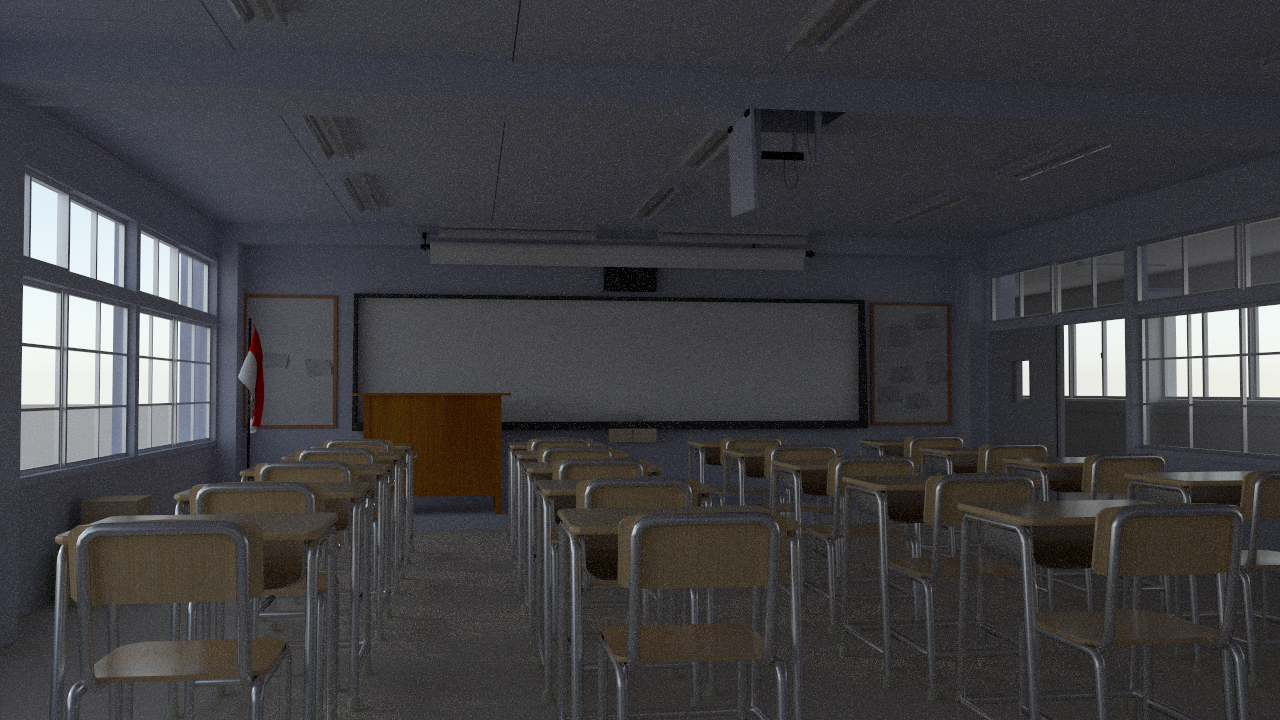
\includegraphics[width=\textwidth]{classroom_naive}
        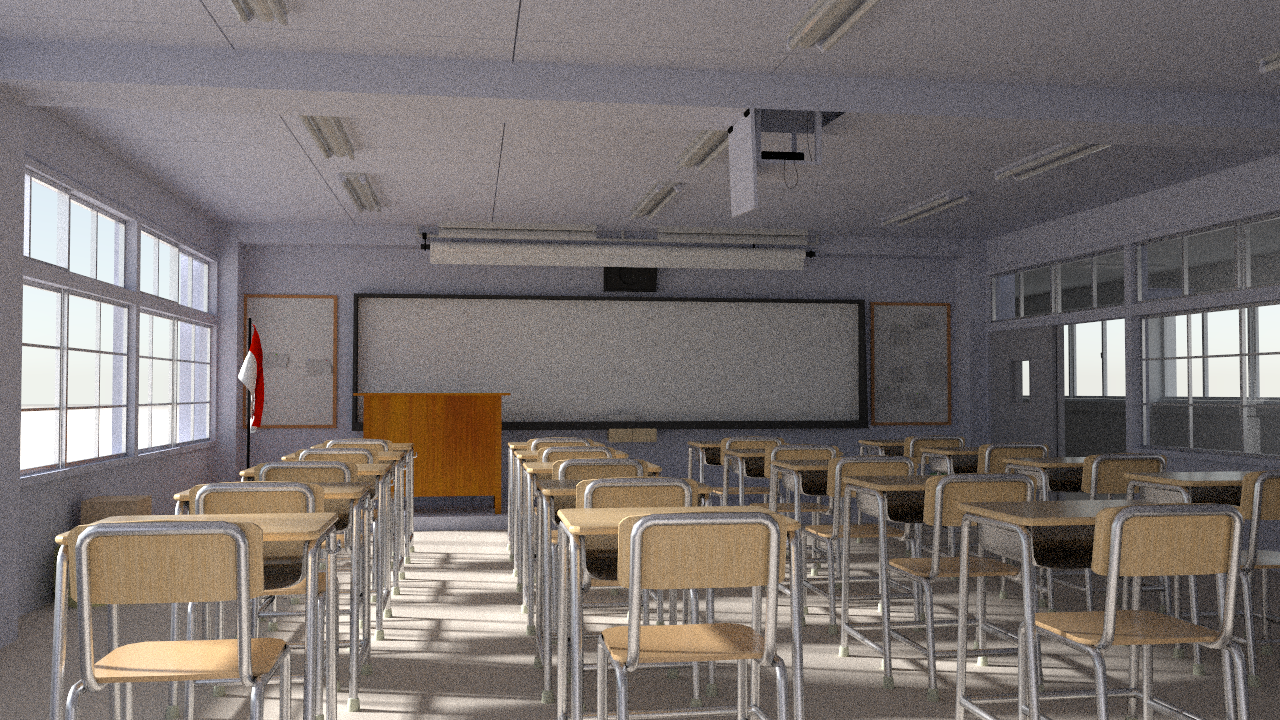
\includegraphics[width=\textwidth]{classroom_path}
        \centering
        \label{fig:classroom}
    \end{figure}

    \begin{figure}[h]
        \caption{there is no difference between naive and light sampling since the only light source is the environment}
        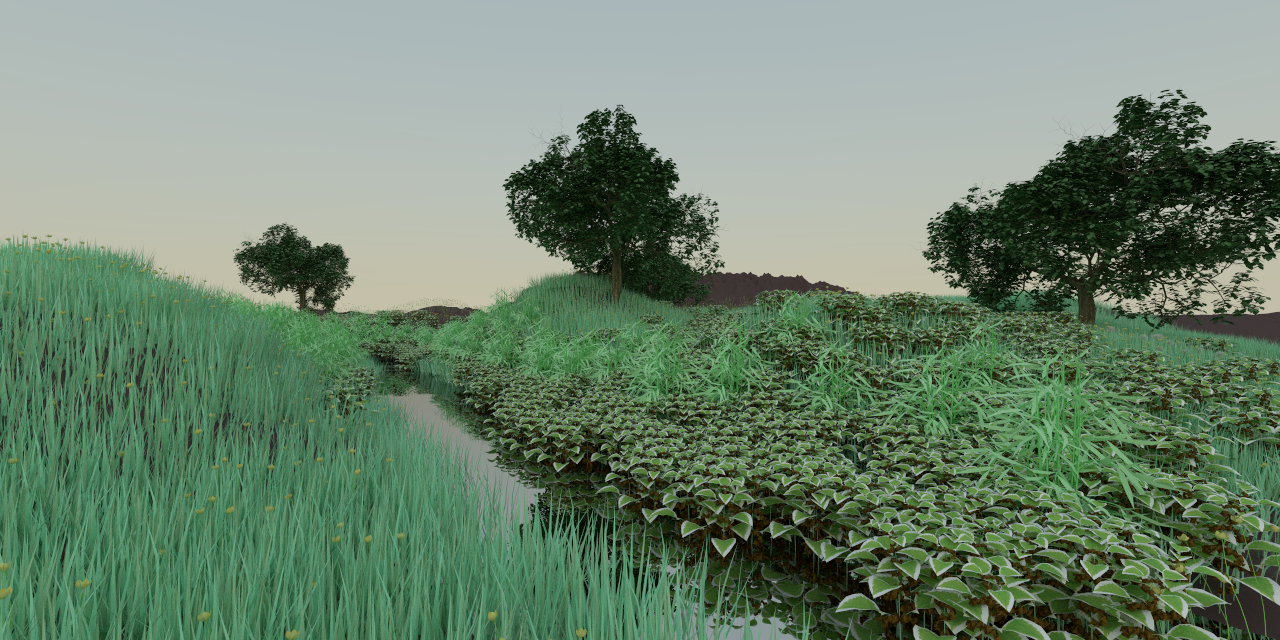
\includegraphics[width=\textwidth]{ecosys_naive}
        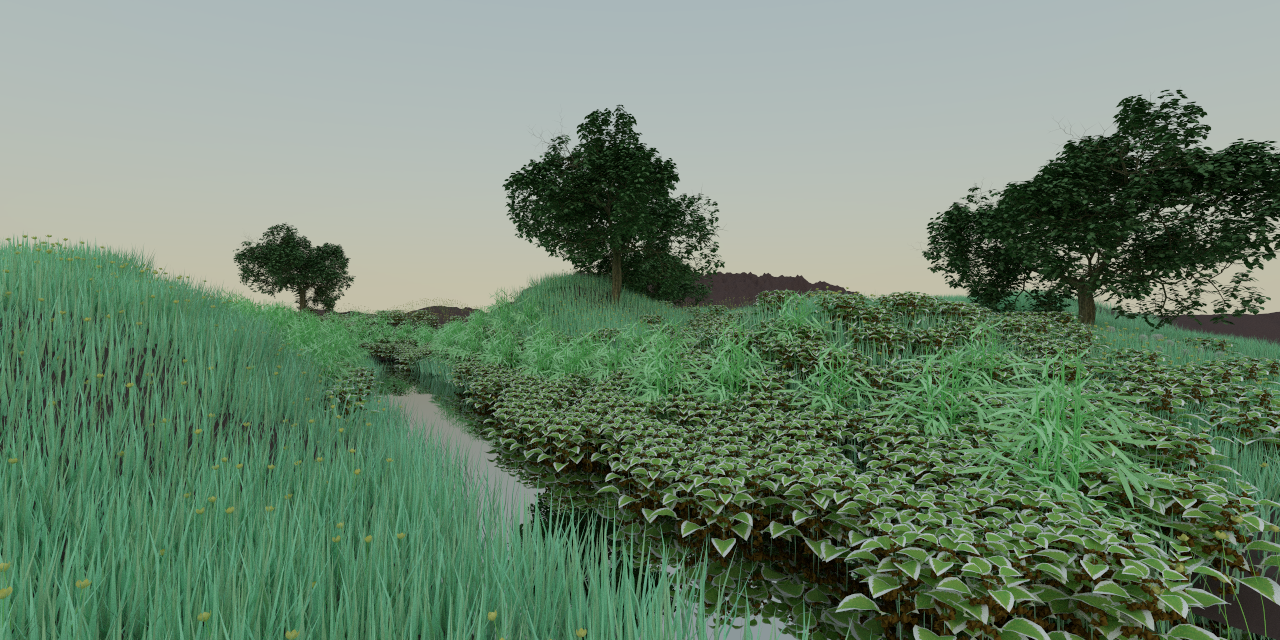
\includegraphics[width=\textwidth]{ecosys_path}
        \centering
        \label{fig:ecosys}
    \end{figure}

    \begin{figure}[h]
        \caption{naive sampling doesn't work with volumes}
        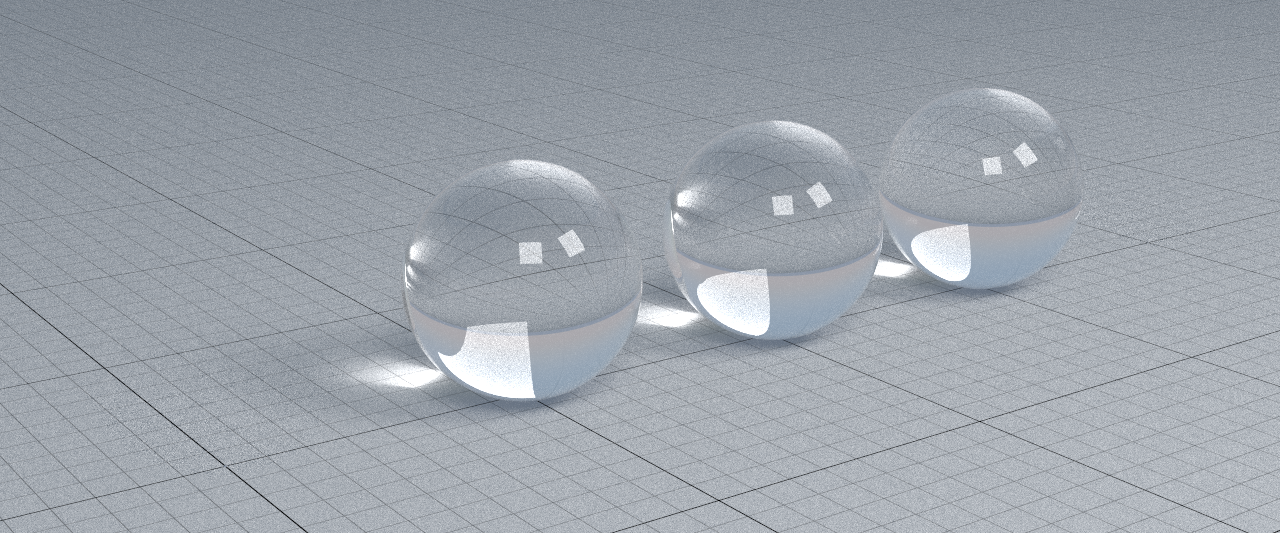
\includegraphics[width=\textwidth]{materials4_naive}
        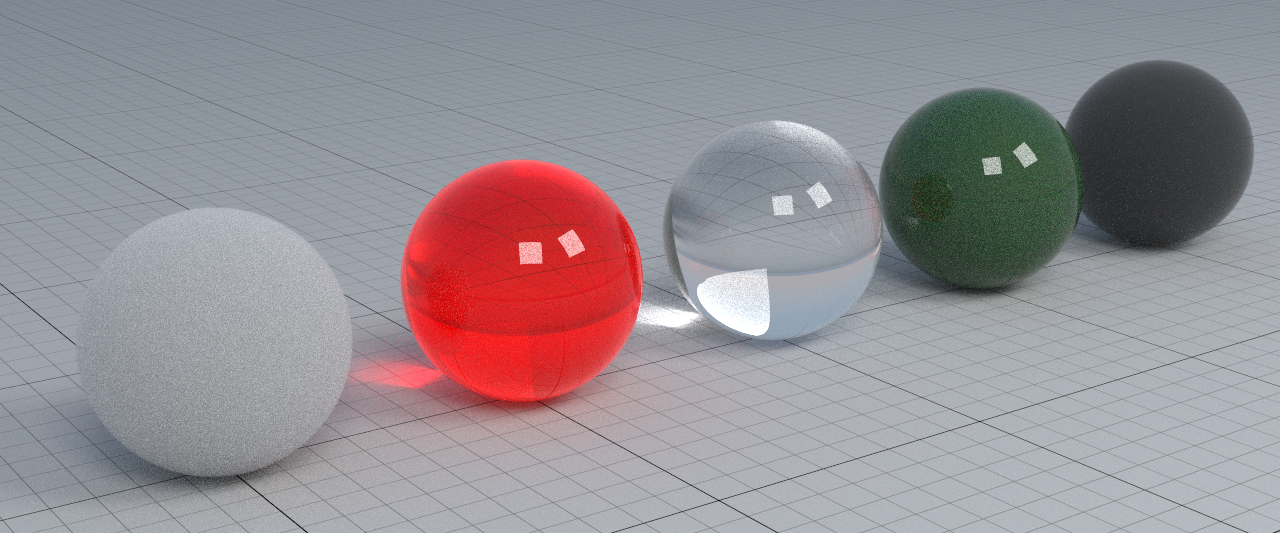
\includegraphics[width=\textwidth]{materials4_path}
        \centering
        \label{fig:materials4}
    \end{figure}


\end{document}